The specification of a polygon surface mesh consists of combinatorial
entities: vertices, edges, and faces, and numerical quantities:
attributes such as vertex positions, vertex normals, texture
coordinates, face colors, etc. The \italic{connectivity} describes the
incidences between elements and is implied by the topology of the
mesh. For example, two vertices or two faces are adjacent if there
exists an edge incident to both.\\

% definition

A \italic{halfedge data structure} is an edge-centered data structure
capable of maintaining incidence informations of vertices, edges and
faces, for example for planar maps, polyhedra, or other orientable,
two-dimensional surfaces embedded in arbitrary dimension. Each edge is
decomposed into two halfedges with opposite orientations. One incident
face and one incident vertex are stored in each halfedge. For each
face and each vertex, one incident halfedge is stored (see
Fig.\ref{fig:halfedge}).

% halfedge

\begin{figure}[htb]
    \centering{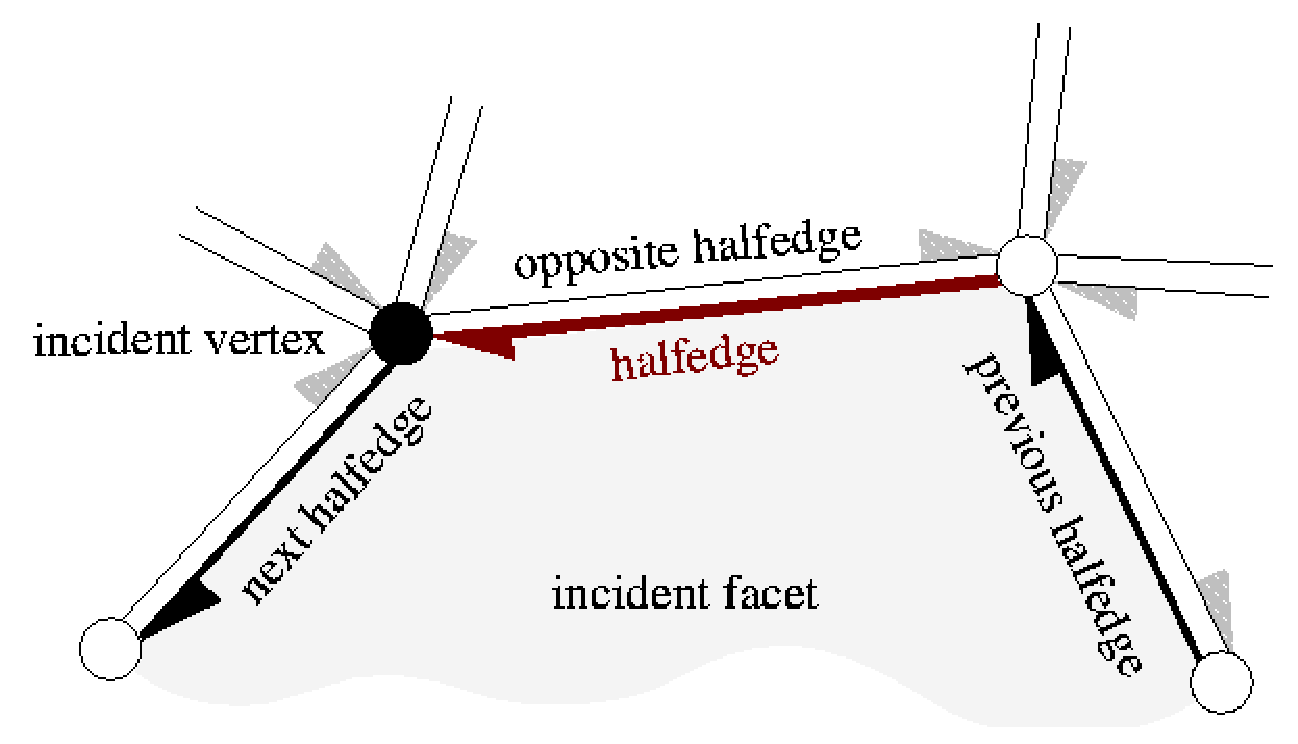
\includegraphics[width=7.0cm]{figs/halfedge}}
    \caption{One halfedge and its incident primitives.}
    \label{fig:halfedge}
\end{figure}
        
Notice that the halfedge data structure is only a combinatorial data
structure, geometric interpretation being added by classes built on
top of the halfedge data structure. On example is the class
\italic{CGAL::Polyhedron\_3} used in this tutorial. The 
halfedge data structure has been very successful for the design of
algorithms on meshes for several reasons:

\begin{itemize}

\item 
an edge-based data structure leads to a constant size structure,
contrary to face-based data structures with inevitable variable
topological structure when dealing with arbitrary vertex valence and
face degrees.

\item 
a halfedge encodes the orientation of an edge, facilitating the mesh
traversal.

\item 
navigation around each vertex by visiting all surrounding edges or
faces is made easy.

\item
each halfedge can be associated with a unique corner, that is a couple
$\{$face,vertex$\}$. The storage of attributes such as normals or
texture coordinates per corner (instead of per vertex) is thus
allowed.

\end{itemize}
